\section{Implementierung des Hopfield Modells}
Für die Implementierung Hopfield Modells in Python wurde eine Klasse erstellt:
\begin{minted}{python}
class HopfieldNetwork:
	def __init__(self, N=100, filepath=None):
		...
\end{minted}
Im Folgenden sind die wichtigsten Funktionen und die Anwendung der \textbf{HopfieldNetwork} Klasse gezeigt werden.
\subsection{Wichtige Funktionen} 
Energiefunktion:
\begin{align}
H = - \frac{1}{2} \sum_{i,j}^{N} w_{ij} S_i S_j
\end{align}
\begin{minted}{python}
def compute_energy(self, S):
    return -0.5 * np.einsum('i,ij,j', S, self.w, S)
\end{minted}
Hebb-Matrix:
\begin{align}
w_{ij} = \frac{1}{N} \sum_{\mu = 1}^{p} \xi_i^{(\mu)} \xi_j^{(\mu)}
\end{align}
\begin{minted}{python}
def construct_hebb_matrix(xi):
	n = xi.shape[0]
	if len(xi.shape) == 1:
		w = np.outer(xi, xi) / n  # p = 1
	elif len(xi.shape) == 2:
		w = np.einsum('ik,jk', xi, xi) / n  # p > 1
	else:
		raise ValueError("Unexpected shape of input pattern xi: {}"\
		.format(xi.shape))
	np.fill_diagonal(w, 0)  # set diagonal elements to zero
return w
\end{minted}
Hamming-Metrik:
\begin{align}
H(x,y) = \# \{i: x_i \neq y_i\}
\end{align}
\begin{minted}{python}
def hamming_distance(x, y):
    return np.sum(x != y)}
\end{minted}

\subsection{Anwendung}
Die \textbf{HopfieldNetwork} Klasse kann wie folgt genutzt werden:\\\\
Erstelle ein neues Hopfield Netz der Größe $N=100$:
\begin{minted}{python}
hopfield_network1 = HopfieldNetwork(N=100)
\end{minted}
Öffne eines bereits trainiertes Hopfield Netz:
\begin{minted}{python}
hopfield_network2 = HopfieldNetwork(filepath='network2.npz')
\end{minted}
Speichere ein Netzwerk als Datei:
\begin{minted}{python}
hopfield_network3.save_network('path/to/file')
\end{minted}
Speichere/Trainiere Bilder ins Hopfield Netz:
\begin{minted}{python}
hopfield_network1.train_pattern(input_pattern)
\end{minted}
Starte ein asynchrones Update mit 5 Iterationen:
\begin{minted}{python}
hopfield_network1.update_neurons(iterations=5, mode='async')
\end{minted}
Berechne die Energiefunktion eines Bildes:
\begin{minted}{python}
hopfield_network1.compute_energy(input_pattern)
\end{minted}



\subsection{Test des Hopfield Modells}
Zum Test der Implementierung wurde ein Hopfield Netz mit 10000 Neuronen initializiert und mit Bildner von 10 bekannten Physikern trainiert. Als Startkonfiguartion wurde einmal ein Teil eines gespeichterten Bilders und einmal eine verrauschte Version eines gespeichterten Bilders gewählt. Danach wurden zwei asynchrone Updates ausgeführt. Die Neuronenkonfigurationen zu den jeweiligen Zeitschritten (und der Hammingabstand zum gespeichtern Bild) sind in \autoref{fig:reconstruct_partial} und in \autoref{fig:reconstruct_randomized} zu sehen.
\begin{figure}[htp]
	\centering
	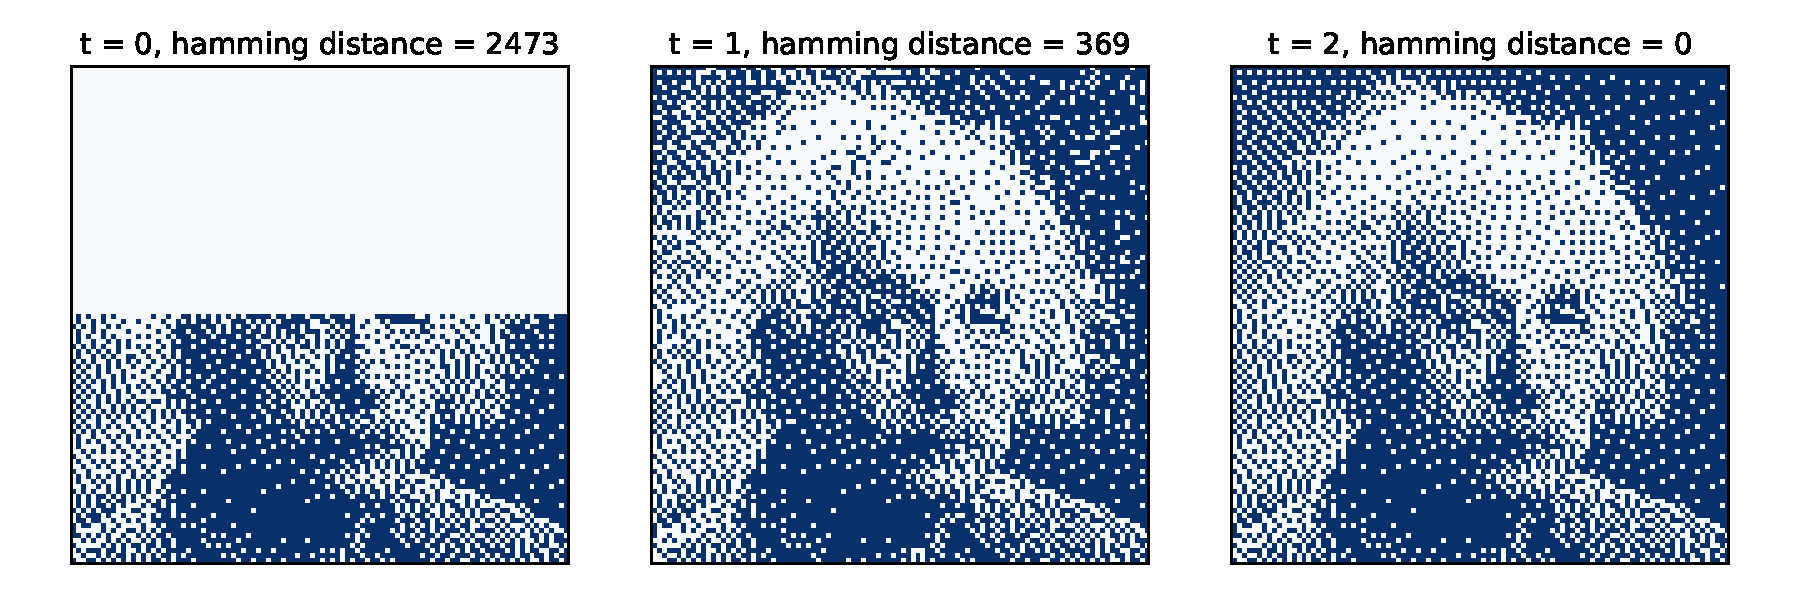
\includegraphics[width = \textwidth]{images/reconstruct_einstein.pdf}
	\caption{Bildrekonstruktion aus einem Teilbild. Für das Hopfield Netzwerk wird ein Teil eines gespeichterten Bildes als Startkonfiguartion der Neuronen gewählt. Nach zwei Iterationen evolviert das Netzwerk zum gespeichert Bild. Der angegebene Hammingabstand bezieht sich dabei auf das gespeicherte Bild.}
	\label{fig:reconstruct_partial}
\end{figure}
\begin{figure}[htp]
	\centering
	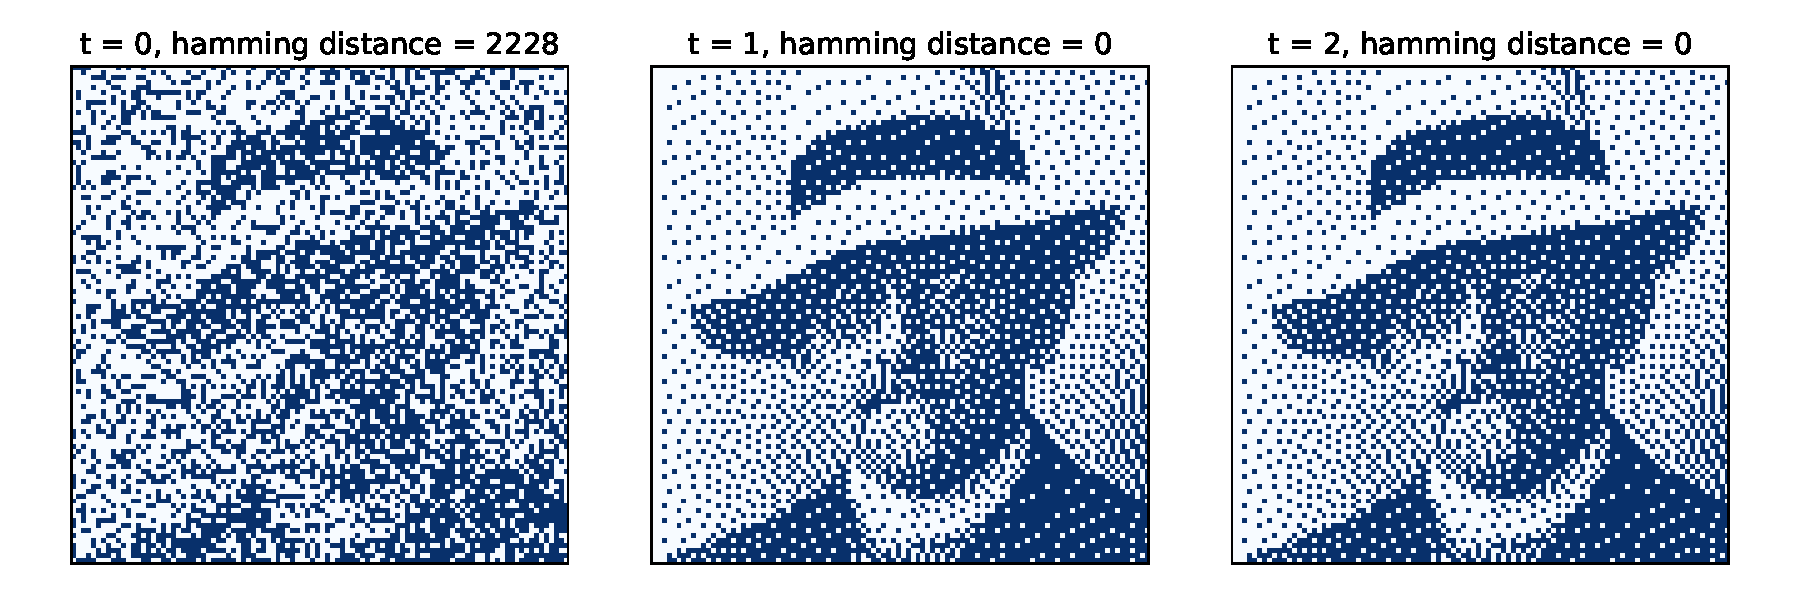
\includegraphics[width = \textwidth]{images/reconstruct_hilbert.pdf}
	\caption{Bildrekonstruktion aus einem verauschtem Bild. Für das Hopfield Netzwerk wird ein verauschte Version eines gespeichterten Bildes als Startkonfiguartion der Neuronen gewählt. Nach zwei Iterationen evolviert das Netzwerk zum gespeichert Bild. Der angegebene Hammingabstand bezieht sich dabei auf das gespeicherte Bild.}
	\label{fig:reconstruct_randomized}
\end{figure}

\clearpage

\subsection{Python GUI} \label{python_gui}
Im Hopfield network GUI werden die eindimensionalen Vektoren der Neuronenzustände als zweidimensionales binäres Bild visualisiert. Der Nutzer hat die Möglichkeit verschiedene Bilder in das Netzwerk zu laden und dieses anschließend asynchron oder synchron mit oder ohne endliche Temperaturen zu aktualisieren. Um die Funktionsweise des Netzes direkt zu prüfen, können im Reiter \textbf{Examples} verschiedene vorgespeichterte Netzwerke (10 Bilder bekannter Physiker, 20 zufällige Muster, ...) geladen werden. Im Folgenden soll ein kurzer Überblick über die Bedienung sowie die möglichen Funktionen des GUIs geschaffen werden.

\begin{figure}[htp]
	\centering
	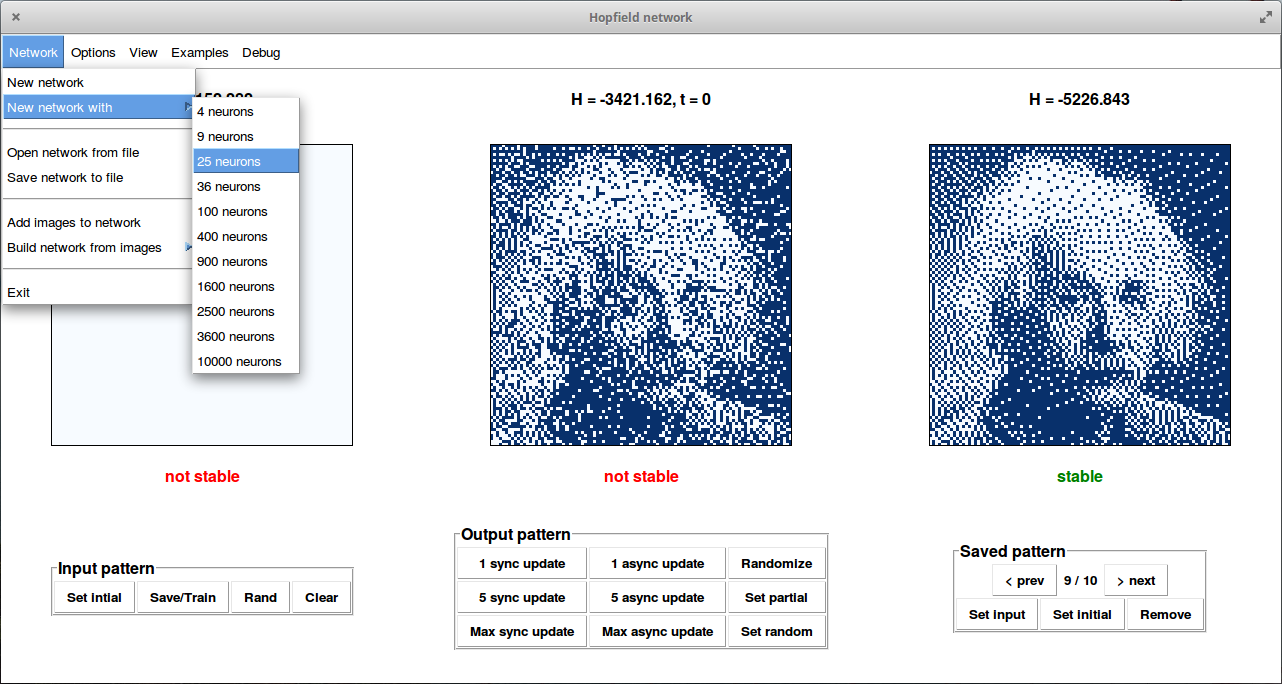
\includegraphics[width = \textwidth]{images/gui_screenshot.png}
	\caption{Screenshot des Hopfield network GUI.}
	\label{fig:gui_screenshot}
\end{figure}

Das Hopfield Network GUI kann mit

\mint{bash}{python3 gui.py}

\noindent gestartet werden. Das Hopfield network GUI lässt sich in 3 sogenannten Frames aufteilen:
\begin{itemize}
\item Der \textbf{Input frame} (links) ist der Hauptinteraktionspunkt mit dem Netzwerk. Der Nutzer hat die Möglichkeit hier ein Inputmuster durch einen Linksklick auf +1, entsprechend durch einen Rechtsklick auf -1 zu setzen. Dies hat erstmal keinen Einfluss auf das Netzwerk. Erst mit den darunter liegenden Buttons kann das Netzwerk verändert werden:
\begin{itemize}
\item \textbf{Set intial} setzt das momentane Inputmuster als Startkonfiguaration der Neuronen.
\item \textbf{Save/Train} speichert/trainiert das momentane Inputmuster in das Hopfield Netz.
\item \textbf{Rand} setzt ein zufälliges Inputmuster.
\item \textbf{Clear} setzt alle Punkte des Inputmusters auf -1.
\end{itemize}
\item Der \textbf{Output frame} (mittig) zeigt die momentane Neuronenkonfiguartion an. Mit den darunter liegenden Buttons kann das Netzwerk asynchron oder synchron aktualisiert werden.
\begin{itemize}
\item \textbf{Sync update} startet ein synchrones Update.
\item \textbf{Async update} startet ein asynchrones Update.
\item \textbf{Randomize} flippt zufällig den Zustand von einem Zehntel der Neuronen.
\item \textbf{Set partial} setzt das erste Hälfte der Neuronen auf -1.
\item \textbf{Set random} setzt einen zufälligen Neuronenzustand.
\end{itemize}
\item Der \textbf{Saved pattern frame} (rechts) bietet die Möglichkeit die bereits im Netzwerk gespeicherten Bilder anzuschauen oder aus dem Netzwerk zu entfernen.
\begin{itemize}
\item \textbf{Set input} setzt das momentan angezeigte Bild als neuen Neuronenzustand.
\item \textbf{Set input} setzt das momentan angezeigte Bild als Inputmuster.
\end{itemize}
\end{itemize}
Menuleiste des GUI:
\begin{itemize}
\item Im Reiter \textbf{Network} kann eine neues Hopfield Netz beliebiger größe initializiert werden. Darüberhinaus besteht die Möglichkeit das momentane Netz zu speichern sowie ein gespeichertes Netz zu laden. Außerdem kann eine Rastergrafik (JPG,PNG,GIF,TIF) in das Netzwerk gespeichert werden oder direkt ein neues Netzwerk aus mehreren Bildern zu erstellen.
\item Im Reiter \textbf{Options} kannd das Update mit endliche Temperaturen (de)aktiviert werden.
\item \textbf{View} bietet einge Möglichkeiten zur optischen Veränderung der GUI.
\item Im Reiter \textbf{Examples} können einige verschieden Beispiel Netze geladen werden.
\end{itemize}




\clearpage